\section{Colors and Light}
\greenbf{CIE Experiment:} subject is shown two stimuli at the same time, one with the pure spectral color, the other a linear combination of the three primaries (RGB). Subject can control how much primaries were dimmed and asked to match the second stimulus to the first. $\rightarrow$ find how humans perceive color. Can also add red light to reference if impossible to match $\rightarrow$ negative red values. \\
\greenbf{xyY color space:} x,y control chormacity, Y is luminance. \\
\vspace{-10pt}
\begin{minipage}{0.4\columnwidth}
    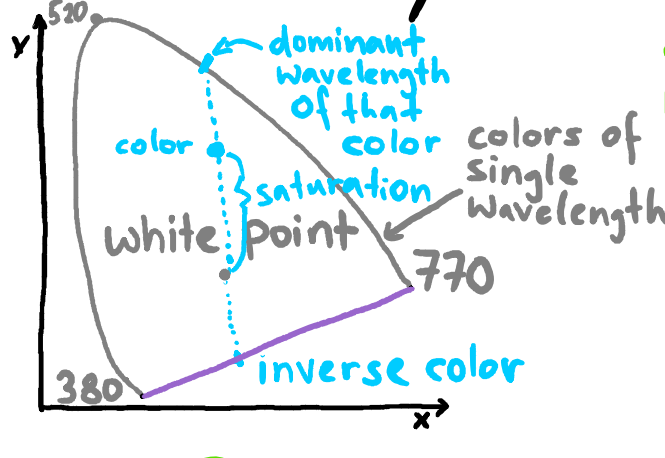
\includegraphics[width=\linewidth]{arjun/cie-chromacity.png}
\end{minipage}%
\begin{minipage}{0.6\columnwidth}
    \greenbf{Color Gamut}
       Linear combination of 3 colors in \(\triangle\).

    \greenbf{Purple Line}
      Non-spectral colors between 380 and 770.

    \greenbf{Dominant Wavelength}
      From color through whitepoint, boundary intersection.

    \greenbf{Saturation}
      Distance from color to white point.

    \greenbf{Isoline}
      Line with constant distance to border (w/o PL).
\end{minipage}
  \vspace{10pt}

\greenbf{RGB \(\to\) XYZ}
  \[\begin{bmatrix}
    \overline{x}(\lambda) \\ \overline{y}(\lambda) \\ \overline{z}(\lambda)
  \end{bmatrix} = \begin{bmatrix}
    2.36 & -0.515 & 0.005 \\ -0.89 & 1.426 & 0.014 \\ -0.46 & 0.088 & 1.009
  \end{bmatrix} \begin{bmatrix}
    \overline{r}(\lambda) \\ \overline{g}(\lambda) \\ \overline{b}(\lambda)
  \end{bmatrix}\]


\greenbf{XYZ \(\to\) xyY}
  \[x = \frac{X}{X + Y + Z} \quad y = \frac{Y}{X + Y + Z} \quad Y = Y \quad \color{H3}X = \frac{xY}{y} \] 
  \[Z = \frac{(1 - x - y)Y}{y}\]


\greenbf{RGB \(\to\) CMY}
  \[\begin{bmatrix}
    C \\ M \\ Y
  \end{bmatrix} = \begin{bmatrix}
    1 \\ 1 \\ 1
  \end{bmatrix} - \begin{bmatrix}
    R \\ G \\ B
  \end{bmatrix}\]


\greenbf{RGB \(\to\) YIQ}
  \[\begin{bmatrix}
    Y \\ I \\ Q
  \end{bmatrix} = \begin{bmatrix}
    0.299 & 0.587 & 0.114 \\ 0.596 & -0.275 & -0.321 \\ 0.212 & -0.523 & 0.311
  \end{bmatrix} \begin{bmatrix}
    R \\ G \\ B
  \end{bmatrix}\]


\greenbf{RGB \(\to\) HSV}
  \vspace{-8pt}
  \lstset{basicstyle=\ttfamily\footnotesize,breaklines=true}
  \begin{center}
    \begin{lstlisting}
  min = min(R, G, B)
  max = max(R, G, B)
  V = max;
  If (max != 0) S = (max - min) / max
  Else S = 0;
  H = Hue (V, S, R, G, B); // proced.
    \end{lstlisting}
  \end{center}

\greenbf{RGB:} Same color space as XYZ. Can be transformed with matrix multiplication. Additive color model, good for combining colored lights. Used in monitors/displays. \\
\greenbf{CMY:} Inverse of RGB. Subtractive color model. Used in passive color systems (printers). \\

\greenbf{YIQ:} Luminance Y, In-phase I (orange-blue), Quadrature Q (purple-green) components. Advantages for natural and skin colors. Used in NTSC US-color TV. \\
\greenbf{HSV:} Hue: base color, Saturation: purity of color, Value: brightness. Intuitive for interactive color picking. Used by designers in Photoshop. \\
\greenbf{Lab:} CIE does not provide perceptually correct distances. The Lab color space is perceptually uniform, meaning that small changes in the euclidean distance correspond to small changes in perceived color.